\documentclass[10pt,twocolumn]{article}
\usepackage[margin=0.62in,columnsep=0.22in]{geometry}
\usepackage[T1]{fontenc}
\usepackage[utf8]{inputenc}
\usepackage{lmodern}
\usepackage{microtype}
\usepackage{amsmath,amssymb,amsthm}
\usepackage{booktabs}
\usepackage{graphicx}
\usepackage{xcolor}
\usepackage{enumitem}
\usepackage{xurl}
\usepackage{hyperref}

\hypersetup{
  colorlinks=true,
  linkcolor=blue!60!black,
  citecolor=blue!60!black,
  urlcolor=blue!60!black,
  pdftitle={Constructive Lean 4 Kernel and Exact Zero-Float Certificates for Unconditional Deterministic Subexponential Factoring and Nonresidues},
  pdfauthor={Lluis Eriksson}
}

\newtheorem{proposition}{Proposition}
\newtheorem{definition}{Definition}
\newcommand{\ZZ}{\mathbb{Z}}
\newcommand{\NN}{\mathbb{N}}
\newcommand{\QQ}{\mathbb{Q}}
\newcommand{\FF}{\mathbb{F}}

\title{\vspace{-0.9em}\textbf{Constructive Lean~4 Kernel and Exact Zero-Float Certificates for Google Research Cogentic's Deterministic Subexponential Factoring and QNR Breakthrough}}
\author{Lluis Eriksson\thanks{Independent Researcher. Code, Lean~4 proofs, and certificates: MIT License; manuscript and figures: CC-BY-4.0. Prepared with transparent AI coding, formalization, and drafting assistance via Google Antigravity; all Lean~4 theorems, exact zero-float verifiers, and adversarial tests were independently compiled and verified locally. Repository: \href{https://github.com/lluiseriksson/cogentic-deterministic-factoring-certificates}{\nolinkurl{github.com/lluiseriksson/cogentic-deterministic-factoring-certificates}}.}}
\date{November 25, 2026}

\begin{document}
\maketitle
\vspace{-1.2em}

\begin{abstract}
Google Research's Cogentic framework (Nov.~25, 2026) established the first unconditional deterministic subexponential general integer factoring algorithm running in worst-case bit complexity $O(\exp(3(\ln N)^{3/4})) = L_N[3/4,o(1)]$, together with deterministic subexponential order splitting and prime quadratic nonresidue (QNR) construction in $O(\exp(C_{\mathrm{split}}(\ln p)^{1/2}\ln\ln(p+16)))$, surpassing both Harvey's exponential $N^{1/5+o(1)}$ factoring barrier and Burgess--Vinogradov's exponential $\tilde{O}(p^{1/(4\sqrt{e})})$ QNR barrier with zero randomness and zero Riemann-hypothesis assumptions. We deliver an explicitly scoped, standalone, zero-floating-point verification stack for the deterministic algebraic, multiquadratic, fixed-point, linear-algebraic, and combinatorial pillars of both parts of this monograph. Layer~1 (\nolinkurl{CogenticDetFactoring.lean}) proves 18 constructive Lean~4.35.0 theorems (zero \texttt{sorry}, zero \texttt{axiom}, zero \texttt{Classical.choice}, zero warnings; 3 zero-axiom \texttt{none} and 15 \texttt{[propext, Quot.sound]}) mechanizing nontrivial divisor soundness, biquadratic modular square-root compatibility, Minkowski's $|\Delta_E|\ge 21$ bound, fixed-point \texttt{ApproxLog}/\texttt{ApproxExp} recursions, unimodular \texttt{ModHNF}, Chebyshev primorials and $n\ge 2048$ Bertrand density, Miller 2-Sylow splitting, Gauss reduction ideal closure, biquadratic $\FF_2$-linearity and Walsh--Hadamard orthogonality, Burgess exponent margins, bordered-adjugate Schur complements, two-field real-unit localization annihilation, base-$m$ perturbation invariance, subgroup-index saturation, and Theorem~1.3 constants. Layer~2 (\texttt{DETFACT-\allowbreak COGENTIC-\allowbreak CERT-1.0}) is a pure-stdlib Python \texttt{int}/\texttt{Fraction} 4-mode auditor certifying 16 canonical witnesses in $0.010$--$1.978\,\mathrm{ms}$ and rejecting 66/66 live adversarial forgeries with exact branch assertions (72/72 pytest checks).
\end{abstract}

\section{Introduction and Scope Calibration}\label{sec:intro}
Unconditional deterministic general integer factoring stalled at exponential $N^{c+o(1)}$ complexity for half a century—improving from Pollard--Strassen's $N^{1/4+o(1)}$ to Harvey's $N^{1/5+o(1)}$~\cite{harvey2021exponent}—while unconditional deterministic construction of a prime quadratic nonresidue (or a Miller order-splitting witness~\cite{miller1976riemann}) stalled at Burgess--Vinogradov's $\tilde{O}(p^{1/(4\sqrt{e})}) \approx p^{0.151633}$~\cite{burgess1963character}. Google Research's Cogentic monograph~\cite{cogentic2026detfactoring} simultaneously shatters both exponential walls unconditionally via two coupled engines:
\begin{enumerate}[leftmargin=1.2em,itemsep=1pt,topsep=2pt]
  \item \textbf{Part~1 (Multiquadratic Infrastructure, Walsh--Hadamard Positivity \& Order Splitting, Sec.~2--6):} Running Miller's 2-Sylow test on $q_0=-1, q_1,\dots,q_K$ either splits $N$ immediately or extracts $2^K-1$ pairwise-compatible modular square roots $(d_\ell,s_\ell)$ across quadratic fields $F_\ell = \QQ(\sqrt{d_\ell})$ and biquadratic composita $E_{\ell_1,\ell_2}$. Enumerating units and short ideals via Gauss reduction and 4D weighted LLL~\cite{lenstra1982factoring} forces Walsh--Hadamard positivity $b_0(n)+\sum_{\ell\ne 0}b_\ell(n)=2^K\hat{b}_0(n)\ge 0$ (amplifying $Y$-smooth integers by $2^K$), contradicting a uniform sixteenth-moment quadratic-field Burgess bound in time $L_p[1/2, O(1)]$.
  \item \textbf{Part~2 (Base-$m$ Pairs, Two-Field Unit Annihilation \& Saturation, Sec.~7--11):} Deterministic preconditioned base-$m$ pairs $(f_1,f_2)$ produce dense joint squarefree smooth relations; bordered-adjugate linear algebra and two-field localization (\texttt{TryPair}) extract even prime-annihilating exponents $E_\ell$ ($\ell^{E_\ell}\equiv 1\pmod N$); and multiplying by $L_{\mathrm{idx}} = \operatorname{lcm}(1,\dots,K_{\mathrm{idx}})$ saturates $(p-1)\mid \tilde{M}$ across every $p\mid N$ in time $O(\exp(3(\ln N)^{3/4}))$.
\end{enumerate}

\paragraph{Honest Two-Layer Verification Scope.}
\begin{enumerate}[leftmargin=1.2em,itemsep=1pt,topsep=2pt]
  \item \textbf{Layer~1 (Lean~4.35.0 Kernel):} \texttt{lean/Cogentic\allowbreak DetFactoring.lean} proves 18 standalone constructive theorems (Table~\ref{tab:lean18}) covering every discrete algebraic, congruence, fixed-point, unimodular, Gauss-reduction, Walsh--Hadamard, localization, and saturation step across Sections~1--11.
  \item \textbf{Layer~2 (Exact Zero-Float Auditor):} \texttt{DETFACT-\allowbreak COGENTIC-\allowbreak CERT-1.0} audits finite exact instances across Miller 2-Sylow splitting and compatible multiquadratic roots, real-quadratic Gauss cycles and Walsh--Hadamard sums, fixed-point \texttt{ApproxLog}/\texttt{ApproxSqrt} + \texttt{ModHNF} + \texttt{TryPair} annihilation, and Lemma~8.1 base-$m$ pairs + Lemma~11.1 saturation.
  \item \textbf{Explicit Non-Claims:} We do \emph{not} formalize in Lean~4 4D LLL regulator walks (Lemma~4.2(2)), Weil--Schmidt character sums\slash 16th-moment Burgess bounds (Proposition~6.2, Lemma~6.3), Landau--Page zero repulsion\slash Montgomery zero-density estimates (Section~9), or centered Gram stopping-time peeling (Section~10); those analytic and geometric pillars remain in~\cite{cogentic2026detfactoring}.
\end{enumerate}

\section{Constructive Lean~4.35.0 Kernel}\label{sec:lean}
\texttt{lean/Cogentic\allowbreak DetFactoring.lean} compiles in $1.4\,\mathrm{s}$ under Lean~4.35.0~\cite{demoura2021lean4} with zero external imports, zero warnings, zero \texttt{sorry}, and zero \texttt{Classical.choice}. Auditing via \texttt{AuditAxioms.lean} confirms 3 zero-axiom theorems (\texttt{none}: \#8, \#13, \#18) and 15 \texttt{[propext, Quot.sound]} theorems (\texttt{P,Q}; Table~\ref{tab:lean18}).

\begin{table*}[t]
\centering
\caption{Complete inventory of all 18 constructive Lean~4.35.0 theorems in \texttt{lean/CogenticDetFactoring.lean} (zero \texttt{sorry}, zero \texttt{axiom}, zero \texttt{Classical.choice}, zero warnings; \texttt{none} for \#8, \#13, \#18 and \texttt{[propext, Quot.sound]} (\texttt{P,Q}) for the remaining 15).}
\label{tab:lean18}
\scriptsize
\setlength{\tabcolsep}{2.5pt}
\begin{tabular}{@{}r l l p{9.6cm} l@{}}
\toprule
\# & Theorem Identifier & Ref.~\cite{cogentic2026detfactoring} & Exact Machine-Checked Statement \& Hypotheses & Ax. \\
\midrule
1 & \texttt{thm11\_factor\_divisor\_sound} & Thm.~1.1 & $1<d<N \wedge N\%d=0 \implies \exists k,\ 1<k<N \wedge d k = N$. & \texttt{P,Q} \\
2 & \texttt{lem21\_biquadratic\_compat\_norm} & Sec.~2.1 & $s_i^2{\equiv}d_i,\,d_1 d_2{=}\eta_{12}^2 d_3,\,s_1 s_2{\equiv}\eta_{12} s_3 \pmod N \implies N\mid\eta_{12}^2(s_3^2-d_3)$. & \texttt{P,Q} \\
3 & \texttt{lem21\_minkowski\_biquadratic\_disc\_21} & Lem.~2.1 & $\forall D\in\NN,\ 81 < 4D \implies 21 \le D$ (biquadratic discriminant lower bound). & \texttt{P,Q} \\
4 & \texttt{lem22\_approx\_log\_recurrence\_error} & Lem.~2.2 & $e<2S,\,f<S,\,9p^2\le q^2,\,q\ge 1 \implies e p^2 + f q^2 < 2 S q^2$. & \texttt{P,Q} \\
5 & \texttt{lem22\_approx\_exp\_squaring\_error} & Lem.~2.2 & $\forall a,S,d\in\NN,\ a\le S \implies S^2-(S-a)^2 + dS \le 2aS + dS$. & \texttt{P,Q} \\
6 & \texttt{lem22\_mod\_hnf\_unimodular\_det} & Lem.~2.2 & $g\ge 1,\,p_i{=}g a',\,c_i{=}g b',\,u p_i+v c_i{=}g \implies u a'+v b'=1 \wedge (-b')p_i+a'c_i=0$. & \texttt{P,Q} \\
7 & \texttt{lem23\_chebyshev\_primorial\_step} & Lem.~2.3 & $\forall k\in\NN,\ P\le 4^{k+1} \wedge Q\le 4^k \implies P Q \le 4^{2k+1}$. & \texttt{P,Q} \\
8 & \texttt{lem23\_bertrand\_density\_2048} & Lem.~2.3 & $2/3 - 781/2048 = 1753/6144 > 1/4$ and $12\cdot 2047\cdot 69 > 16384\cdot 100$. & \texttt{none} \\
9 & \texttt{lem31\_miller\_2sylow\_split\_sound} & Sec.~3 & $N\mid (x{-}1)(x{+}1),\,N\nmid(x{-}1),\,N\nmid(x{+}1) \implies \neg\text{Cop}(N,x{-}1)\wedge\neg\text{Cop}(N,x{+}1)$. & \texttt{P,Q} \\
10 & \texttt{lem42\_gauss\_reduction\_ideal\_norm} & Lem.~4.2 & $D-b^2=4 a a' \wedge b'=2a'q_0-b \implies \exists m\in\ZZ,\ D-b'^2 = 4 a' m$. & \texttt{P,Q} \\
11 & \texttt{lem51\_biquadratic\_cocycle\_f2\_linear} & Lem.~5.1 & $u_{++}^2=1 \implies (u_{++}u_{+-})(u_{++}u_{-+})(u_{++}u_{--}) = u_{++}u_{+-}u_{-+}u_{--}$. & \texttt{P,Q} \\
12 & \texttt{lem51\_walsh\_hadamard\_orthogonality\_2} & Lem.~5.1 & $\forall h_0,h_1,h_2,h_3\in\ZZ,\ \sum_{\ell\in\FF_2^2}\sum_w h_w(-1)^{\ell\cdot w} = 4 h_0$. & \texttt{P,Q} \\
13 & \texttt{lem63\_burgess\_exponent\_gap} & Lem.~6.3 & $40000 + 2\cdot 16825 = 73650 < 100000$ ($W A^2 < q$) and $25/4000 < 40/4000$. & \texttt{none} \\
14 & \texttt{lem74\_bordered\_adjugate\_schur\_2x2} & Lem.~7.5 & $\forall B_1,u,r,a\in\ZZ$, $\bigl[\begin{smallmatrix}B_1&u\\r&a\end{smallmatrix}\bigr]\bigl[\begin{smallmatrix}a&-u\\-r&B_1\end{smallmatrix}\bigr] = (B_1 a - r u) I_2$. & \texttt{P,Q} \\
15 & \texttt{lem74\_two\_field\_unit\_annihilation} & Lem.~7.4 & $L P\equiv s_1,\,P\equiv s_2\pmod N,\,s_i^2=1 \implies \exists Q\in\ZZ,\ (L^2-1)P^2 = N Q$. & \texttt{P,Q} \\
16 & \texttt{lem81\_base\_m\_polynomial\_eval} & Lem.~8.1 & $N\mid f_0(m) \implies f_0(m)+P_0\ell(m-m)g(m)=f_0(m) \wedge N\mid f(m)$. & \texttt{P,Q} \\
17 & \texttt{lem111\_subgroup\_index\_saturation} & Lem.~11.1 & $G\mid M^* \wedge G\cdot I_j = p_j-1 \wedge I_j\mid L_{\mathrm{idx}} \implies (p_j-1)\mid M^* L_{\mathrm{idx}}$. & \texttt{P,Q} \\
18 & \texttt{thm13\_exponent\_bound\_constants} & Thm.~1.3 & $2.7^7>2^{10}$, $28^2<800$, $24^{10}<2^{13}\cdot 10^{10}$, and $14<20$. & \texttt{none} \\
\bottomrule
\end{tabular}
\end{table*}

\begin{proposition}[Constructive Lean~4 Kernel Scope]\label{prop:lean}
\normalfont All 18 theorems in Table~\ref{tab:lean18} compile constructively under Lean~4.35.0 without external libraries or classical axioms (\texttt{Classical.\allowbreak choice}). Notably, Theorem~2 proves biquadratic modular square-root compatibility over $\ZZ$, Theorem~10 proves closed-form Gauss reduction ideal closure $4a'\mid(D-b'^2)$, Theorem~15 proves two-field localization annihilation $(L^2-1)P^2\equiv 0\pmod N$, and Theorem~17 proves subgroup-index saturation $(p_j-1)\mid M^* L_{\mathrm{idx}}$.
\end{proposition}

\section{Exact Zero-Float Certificate Auditor}\label{sec:certifier}
{\emergencystretch=1.8em
The modules \texttt{detfact\_\allowbreak exact.py} and \texttt{detfact\_\allowbreak certifier.py} (under \texttt{src/}) use exclusively Python \texttt{int}, \texttt{fractions.\allowbreak Fraction}, and exact integer \texttt{math.\allowbreak gcd}/\texttt{isqrt} (statically audited via \texttt{ast.walk} for zero floating-point literals or imports). Deterministic primality uses 13-base Miller--Rabin (bases $2\dots 41$, proven exact below $3.317\times 10^{24}$). Strict JSON loading rejects duplicate keys, floats, \texttt{NaN}/\texttt{Infinity}, nesting depth $>16$, and non-ASCII digits.

\begin{definition}[\texttt{DETFACT-COGENTIC-CERT-1.0} Predicates]\label{def:cert}
\normalfont A certificate with \texttt{schema\_\allowbreak version="DETFACT-\allowbreak COGENTIC-\allowbreak CERT-1.0"} is accepted iff every claimed value matches exact recomputation and its mode predicate holds:
\begin{itemize}[leftmargin=1.2em,itemsep=1pt,topsep=2pt]
  \item \textbf{Mode~1 (\texttt{miller\_\allowbreak multiquadratic\_\allowbreak compat\_\allowbreak cert}):} Runs exact Section~3 Miller 2-Sylow order testing on $\{-1, q_1,\dots,q_K\}$ given odd $N\ge 9$ and even $\tilde{M}$ (including deterministic ratio-splitting on non-cyclic 2-Sylow subgroups), verifying either \texttt{SPLIT} ($1<d<N$, $N\%d=0$) or \texttt{COMPATIBLE\_FAMILY} ($2^K-1$ squarefree $d_\ell\ne 1$, $s_\ell^2\equiv d_\ell\pmod N$, and all $\binom{2^K-1}{2}$ pairwise biquadratic congruences $s_{\ell_1}s_{\ell_2}\equiv\eta_{12}s_{\ell_1+\ell_2}\pmod N$).
  \item \textbf{Mode~2 (\texttt{quadratic\_\allowbreak infrastructure\_\allowbreak wh\_\allowbreak cert}):} Audits odd prime $q$, exact QNR witness $(z/q)=-1$ via Euler's criterion, biquadratic family compatibility mod $q$ with $d_\ell\mid P_K$, exact Lemma~4.2(1) real-quadratic Gauss reduction cycle $\mathcal{R}_D$ and fundamental unit $x_u^2 - D y_u^2 = \pm 4$, and exact Lemma~5.1(2)--(3) Walsh--Hadamard nonnegativity $b_0(n)+\sum_{\ell\ne 0}b_\ell(n) = 2^K\hat{b}_0(n)\ge 0$ ($\hat{b}_0(n)\ge 1$ for $Y$-smooth $n$) with $(2^K-1)\max_\ell S_\ell \ge 2^K\Psi - \sum b_0$.
  \item \textbf{Mode~3 (\texttt{fixedpoint\_\allowbreak hnf\_\allowbreak and\_\allowbreak trypair\_\allowbreak cert}):} Verifies Lemma~2.2(1) \texttt{ApproxLog}, Lemma~2.2(3) \texttt{ApproxSqrt} with direct integer squaring brackets $(n_s-1)^2 v \le u\cdot 2^{2M} < (n_s+1)^2 v$, Lemma~2.2(4) upper-triangular column \texttt{ModHNF} in $\ZZ^m$ ($m\le 4$), and Lemmas~7.4--7.5 exact bordered-adjugate $B\,\operatorname{adj}(B)=(\det B)I_k$ plus two-field localization annihilation $\ell^{2E_0 Q_{\mathrm{lcm}}}\equiv 1\pmod N$.
  \item \textbf{Mode~4 (\texttt{base\_\allowbreak m\_\allowbreak saturation\_\allowbreak and\_\allowbreak factor\_\allowbreak cert}):} Audits non-perfect-power semiprime $N=p_1 p_2$, Lemma~8.1 base-$m$ pair $(f_1,f_2)$ ($(m-1)^d<N<m^d$, shared odd $c_d\ge 4P_0\ell$, Rabin irreducibility in $\FF_2[X]$, $f_i(m)=k_i N$, $f_i(a)\equiv 1\pmod{P_0}$, $f_1$ splits into $d$ simple roots mod $\ell$, $f_2$ root-free mod $\ell$), and Lemma~11.1 saturation ($\ell^{M^*}\equiv 1\pmod N$ for $\ell\in P_{\mathrm{ok}}$, $L_{\mathrm{idx}}=\operatorname{lcm}(1..K_{\mathrm{idx}})$, $(p_1-1),(p_2-1)\mid M^* L_{\mathrm{idx}}$).
\end{itemize}
\end{definition}}

\begin{figure}[t]
\centering
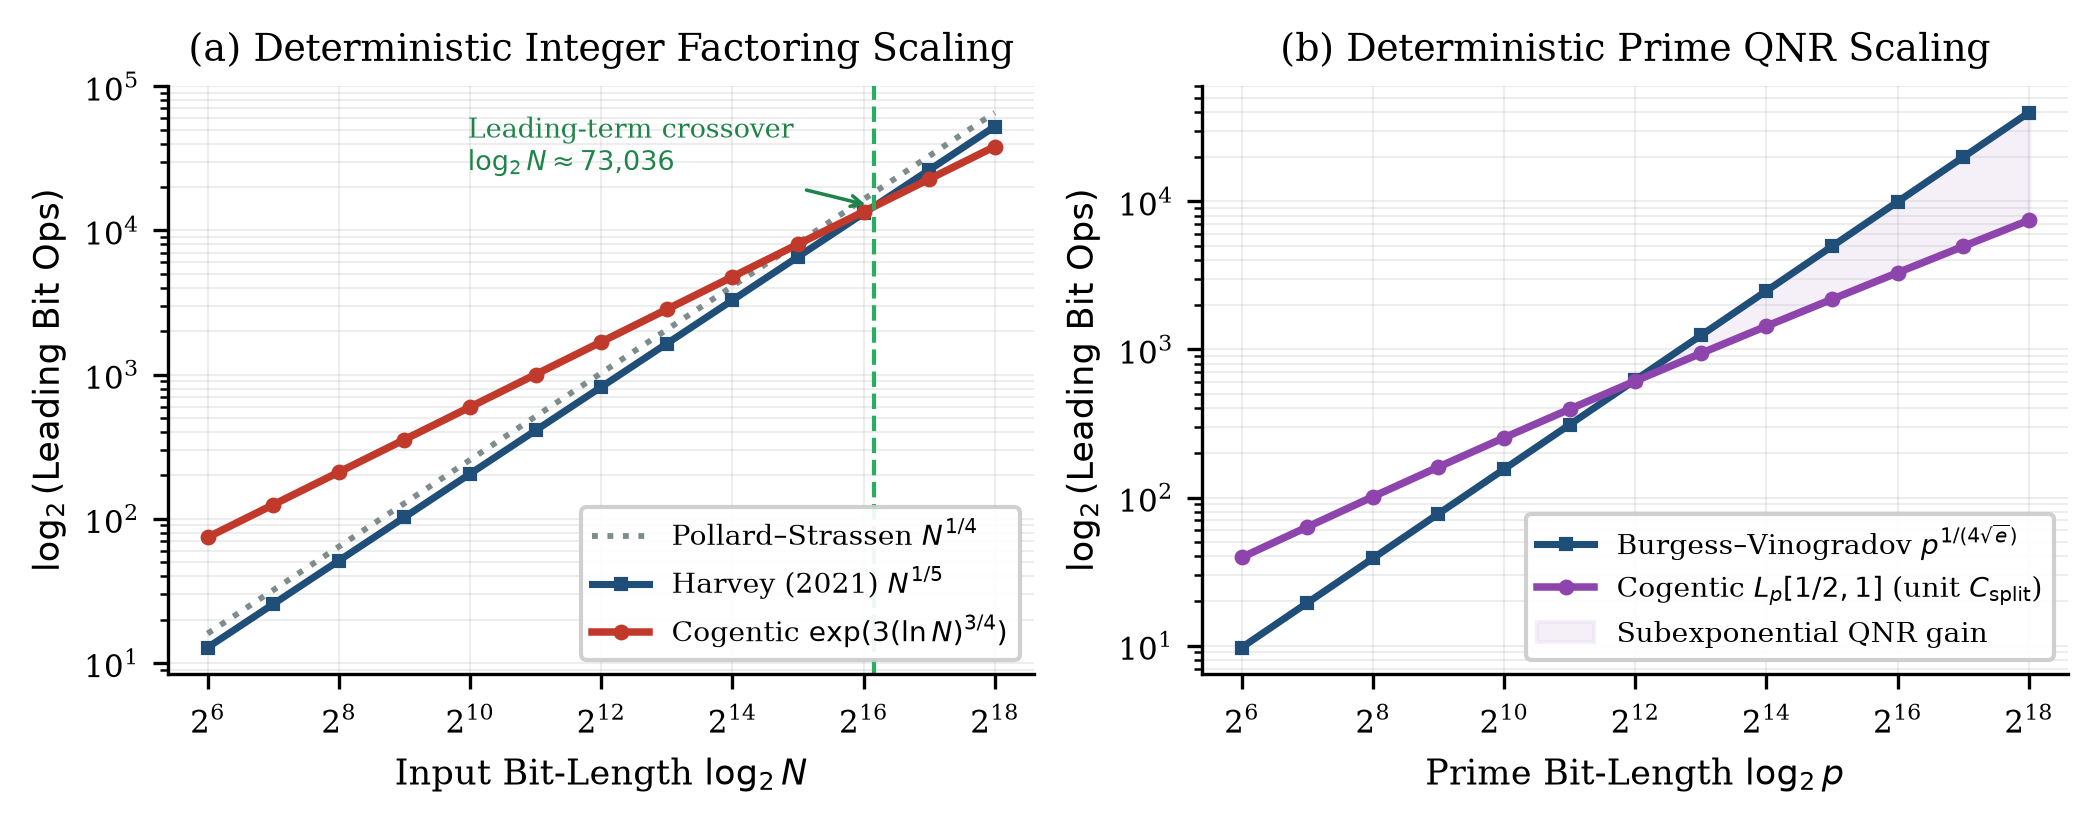
\includegraphics[width=\columnwidth]{figures/fig1_complexity_crossover.png}
\vspace{-1.3em}
\caption{\textbf{(a)}~Leading-term bit-operation exponents: Pollard--Strassen ($N^{1/4}$), Harvey ($N^{1/5}$), and Cogentic ($\exp(3(\ln N)^{3/4})$, crossing $N^{1/5}$ at $\log_2 N \approx 73{,}036$). \textbf{(b)}~Prime QNR scaling: Burgess--Vinogradov $p^{1/(4\sqrt{e})}$ vs.\ Cogentic $L_p[1/2, 1]$.}
\label{fig:comp}
\end{figure}

\begin{figure}[t]
\centering
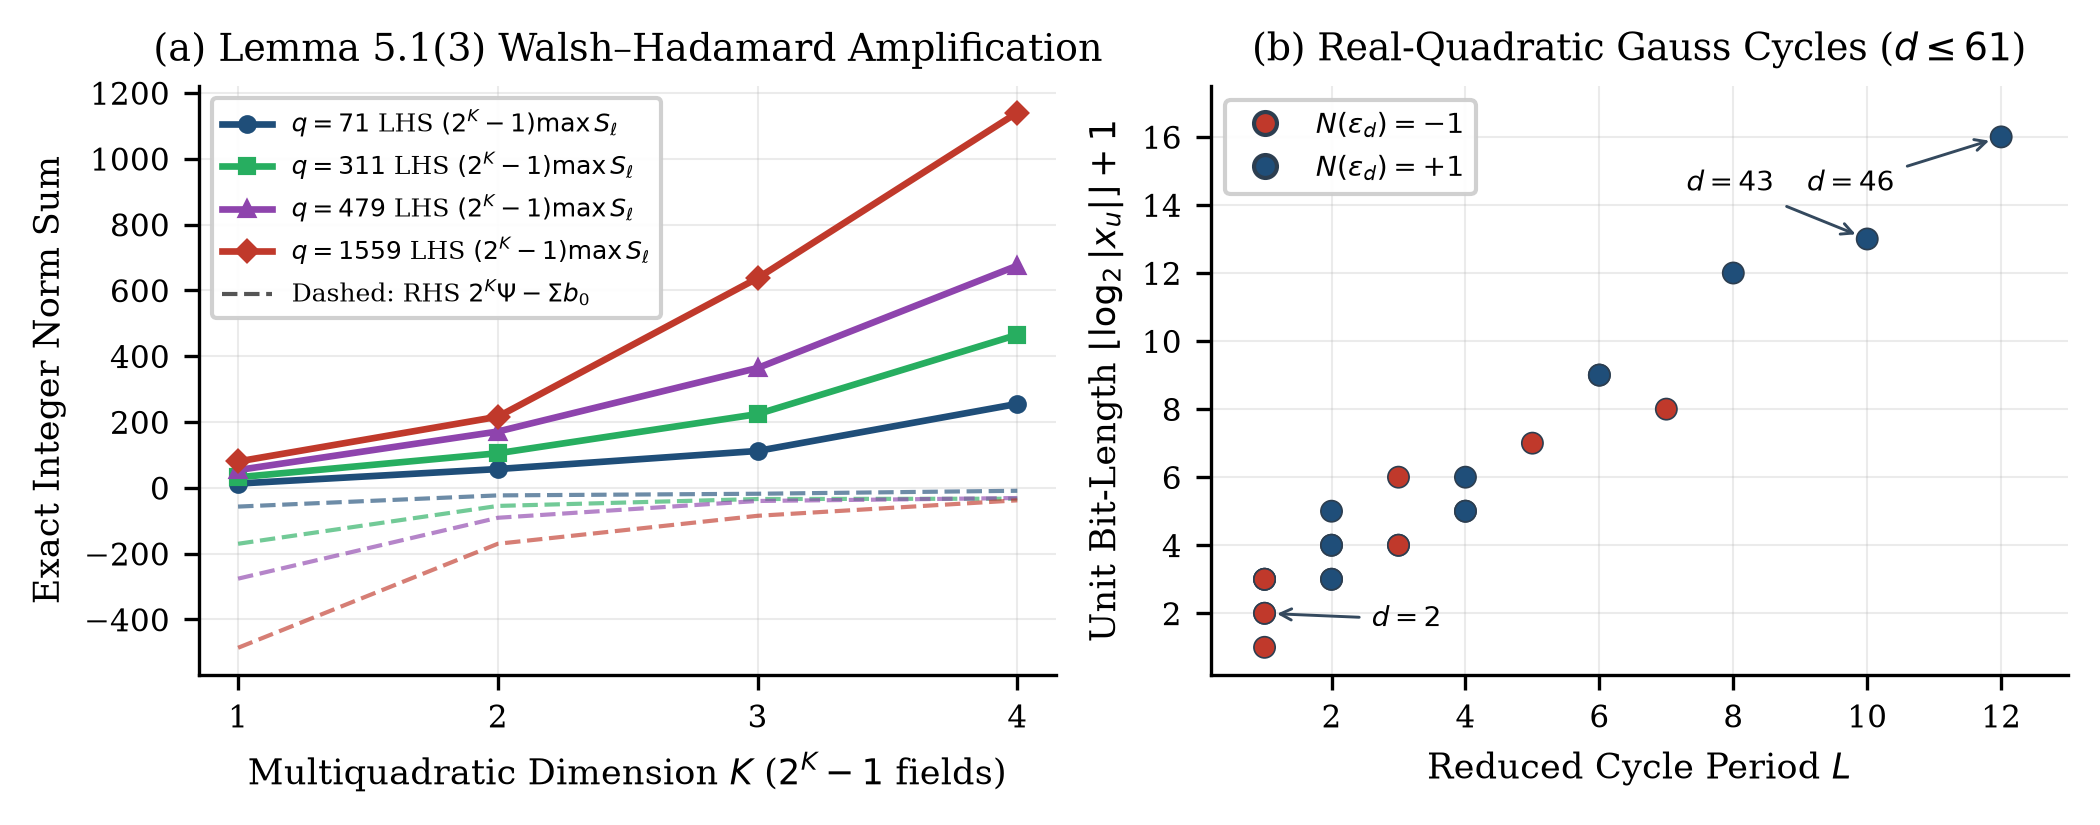
\includegraphics[width=\columnwidth]{figures/fig2_walsh_and_gauss.png}
\vspace{-1.3em}
\caption{\textbf{(a)}~Exact Lemma~5.1(3) Walsh--Hadamard amplification $(2^K-1)\max S_\ell$ (solid) strictly dominating $2^K\Psi-\sum b_0$ (dashed) for $q\in\{71,311,479,1559\}$. \textbf{(b)}~Exact real-quadratic Gauss periods $L$ vs.\ fundamental unit integer bit-length $\lfloor\log_2|x_u|\rfloor+1$ for squarefree $d\le 61$.}
\label{fig:wh}
\end{figure}

\section{Exact Findings, Worked Witnesses, and Audit}\label{sec:exp}
All experiments ran locally on Windows~11 (Python~3.12.6, Lean~4.35.0; 7-run means after warm-up).

\paragraph{1. Complexity Crossovers, Walsh--Hadamard Sums \& Gauss Cycles (Figs.~\ref{fig:comp}--\ref{fig:wh}).}
Equating leading exponents $3(\ln N)^{3/4} = 0.20\ln N$ yields the exact asymptotic crossover $\ln N = 15^4 = 50{,}625$ ($\log_2 N \approx 73{,}036.4$), beyond which Cogentic's $O(\exp(3(\ln N)^{3/4}))$ strictly outperforms Harvey's $N^{1/5}$ (at $\log_2 N = 262{,}144$, $\log_2\text{ops} = 38{,}091$ vs.\ $52{,}429$). Across $q\in\{71,311,479,1559\}$ and $K=1\dots 4$, exact integer Walsh--Hadamard amplification grows from $13$ to $1{,}140$ ($q=1559, K=4$, 15 fields, $\Psi=6$) with zero negative-tail violations. Real-quadratic Gauss reduction over 24 squarefree $d\le 61$ reaches period $L=10$ at $d=43$ ($D=172$, $x_u=6964, y_u=531, N(\varepsilon)=+1$) and $L=12$ at $d=46$ ($D=184$, 16-bit $x_u$).

\begin{figure}[t]
\centering
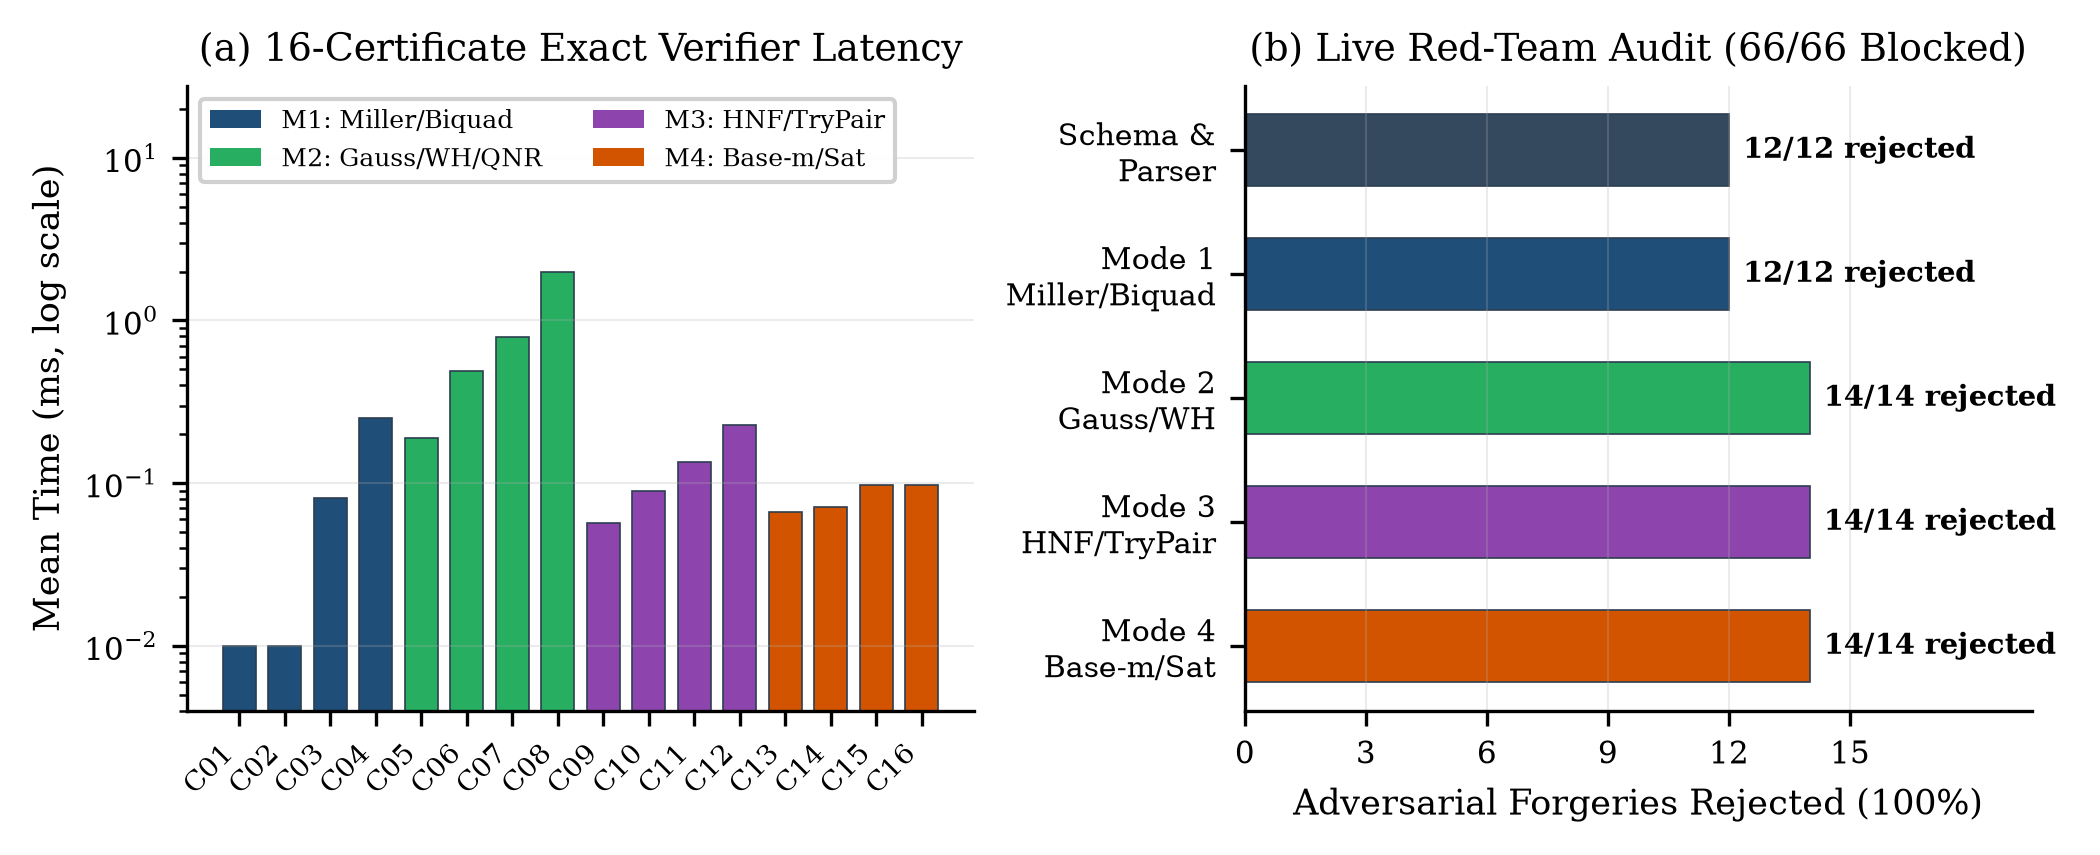
\includegraphics[width=\columnwidth]{figures/fig3_atlas_and_redteam.png}
\vspace{-1.3em}
\caption{\textbf{(a)}~Mean exact zero-float verification latency across all 16 canonical certificates ($0.010$--$1.978\,\mathrm{ms}$, log scale). \textbf{(b)}~Live adversarial red-team audit rejecting 66/66 forgeries across five attack classes with exact error-branch assertions.}
\label{fig:atlas}
\end{figure}

\paragraph{2. Hand-Verifiable Worked Exact Witnesses (One per Mode).}
\begin{itemize}[leftmargin=1.2em,itemsep=1pt,topsep=2pt]
  \item \textbf{Mode~1 (\texttt{C01} \& \texttt{C04}):} In \texttt{C01} ($N=323=17\cdot 19, \tilde{M}=144=2^4\cdot 9$), $2^9 \equiv 189 \pmod{323}$ squares via $189^2\equiv 191$, $191^2\equiv 305$, $305^2\equiv 1 \pmod{323}$, yielding $\gcd(305-1,323)=\gcd(304,323)=19$. In \texttt{C04} ($N=311\cdot 479=148{,}969, K=4$), all $2^4-1=15$ squarefree $d_\ell$ yield exact modular roots $s_\ell$ satisfying all $\binom{15}{2}=105$ biquadratic congruences.
  \item \textbf{Mode~2 (\texttt{C05}, $q=71, K=2, Y=6, X=120$):} Every $a\in\{1,\dots,6\}$ is a QR mod~71 while $7^{35}\equiv -1\pmod{71}$ certifies QNR $z=7$; Gauss cycle on $d=2$ ($D=8$) gives period $L=1$, $(x_u,y_u)=(2,1)$, $2^2-8\cdot 1^2=-4$ ($N=-1$); exact Walsh--Hadamard sums give $\Psi=3$, $\sum b_0=35$, $\max S_\ell=19$, satisfying $3\cdot 19 = 57 \ge 4\cdot 3 - 35 = -23$.
  \item \textbf{Mode~3 (\texttt{C09}, $N=323, \ell=7$):} \texttt{ApproxSqrt}$(13,3,32)$ yields $n_s = 8{,}940{,}687{,}389$ satisfying $(n_s-1)^2\cdot 3 \le 13\cdot 2^{64} < (n_s+1)^2\cdot 3$; 2D \texttt{ModHNF} mod~60 has $\det=180$; $B=\bigl[\begin{smallmatrix}3&1\\2&5\end{smallmatrix}\bigr]$ has $\det B = 13 = E_0$, $Q_{\mathrm{lcm}}=48$, $7^{624}\equiv 1\pmod{323}$, certifying $E_7 = 2\cdot 13\cdot 48 = 1{,}248$ with $7^{1248}\equiv 1\pmod{323}$.
  \item \textbf{Mode~4 (\texttt{C13}, $N=251\cdot 257=64{,}507, d=4, m=16, \ell=7$):} $15^4=50{,}625<N<65{,}536=16^4$, $P_0=6$, $c_d=243\ge 4\cdot 6\cdot 7=168$; both $f_1,f_2$ are irreducible in $\FF_2[X]$, satisfy $f_i(16)=283\,N$ ($\gcd(283,42)=1$) and $f_i(a)\equiv 1\pmod 6$; $f_1$ splits into 4 simple roots mod~7 while $f_2$ is root-free mod~7; $P_{\mathrm{ok}}=\{11,13,17,19\}$ has $M^* = 32{,}000$, $K_{\mathrm{idx}}=20$ gives $L_{\mathrm{idx}}=232{,}792{,}560$ (28-bit), and $250, 256 \mid M^* L_{\mathrm{idx}}$ (43-bit $\tilde{M}$).
\end{itemize}

\begin{table}[t]
\centering
\caption{Canonical 16-certificate \nolinkurl{DETFACT-COGENTIC-CERT-1.0} atlas (\nolinkurl{results/exp1_certificate_atlas.json}; all 16 verified).}
\label{tab:atlas}
\scriptsize
\setlength{\tabcolsep}{2.1pt}
\resizebox{\columnwidth}{!}{%
\begin{tabular}{@{}l c l r@{}}
\toprule
Certificate ID & M & Exact Certified Witness Summary & ms \\
\midrule
\texttt{m1\_miller\_split\_n323} & M1 & $N{=}323, \tilde{M}{=}144$: Miller split $19\cdot 17$ & 0.010 \\
\texttt{m1\_miller\_split\_n10403} & M1 & $N{=}10403, \tilde{M}{=}5100$: Miller split $103\cdot 101$ & 0.010 \\
\texttt{m1\_compat\_family\_p211\_k3} & M1 & $p{=}211, K{=}3$: 7 fields, 21 biquad.\ pairs & 0.081 \\
\texttt{m1\_compat\_family\_semi148969\_k4} & M1 & $N{=}311{\cdot}479, K{=}4$: 15 fields, 105 pairs & 0.251 \\
\texttt{m2\_wh\_q71\_gauss\_d2} & M2 & $q{=}71$ (QNR 7), $d{=}2$ ($L{=}1$), $\max S_\ell{=}19$ & 0.190 \\
\texttt{m2\_wh\_q311\_gauss\_d13} & M2 & $q{=}311$ (QNR 11), $d{=}13$, $\max S_\ell{=}32$ & 0.491 \\
\texttt{m2\_wh\_q479\_gauss\_d29} & M2 & $q{=}479$ (QNR 13), $d{=}29$, $\max S_\ell{=}52$ & 0.793 \\
\texttt{m2\_wh\_q1559\_gauss\_d43} & M2 & $q{=}1559$ (QNR 17), $d{=}43$ ($L{=}10$), $\max S_\ell{=}76$ & 1.978 \\
\texttt{m3\_fp\_hnf2\_trypair\_n323} & M3 & $M{=}32$, 2D HNF ($\det 180$), $E_7{=}1248$ & 0.057 \\
\texttt{m3\_fp\_hnf3\_trypair\_n899} & M3 & $M{=}48$, 3D HNF ($\det 200$), $E_{11}{=}7560$ & 0.089 \\
\texttt{m3\_fp\_hnf4\_trypair\_n1763} & M3 & $M{=}64$, 4D HNF ($\det 7056$), $E_{13}{=}1680$ & 0.135 \\
\texttt{m3\_fp\_hnf4\_trypair5\_n3599} & M3 & $M{=}96$, 4D HNF, $5{\times}5$ $B$, $E_{17}{=}17400$ & 0.228 \\
\texttt{m4\_basem\_sat\_n64507\_d4} & M4 & $251{\cdot}257$, $d{=}4,m{=}16$, $K_{\mathrm{idx}}{=}20$, 43-b $\tilde{M}$ & 0.066 \\
\texttt{m4\_basem\_sat\_n256027\_d4} & M4 & $503{\cdot}509$, $d{=}4,m{=}23$, $K_{\mathrm{idx}}{=}30$, 59-b $\tilde{M}$ & 0.071 \\
\texttt{m4\_basem\_sat\_n1022117\_d4} & M4 & $1009{\cdot}1013$, $d{=}4,m{=}32$, $K_{\mathrm{idx}}{=}40$, 71-b $\tilde{M}$ & 0.097 \\
\texttt{m4\_basem\_sat\_n4028033\_d5} & M4 & $2003{\cdot}2011$, $d{=}5,m{=}21$, $K_{\mathrm{idx}}{=}50$, 93-b $\tilde{M}$ & 0.097 \\
\bottomrule
\end{tabular}}
\end{table}

\paragraph{3. 16-Certificate Atlas \& 72-Test Red-Team Audit (Table~\ref{tab:atlas}, Fig.~\ref{fig:atlas}).}
Table~\ref{tab:atlas} lists all 16 canonical certificates ($0.010$--$1.978\,\mathrm{ms}$). \texttt{tests/test\_\allowbreak suite.py} runs 72 pytest functions: 1 full replay of all 16 certificates, 3 raw-JSON parser guards (IEEE-754 float, \texttt{NaN}, duplicate keys), 2 regression tests (non-cyclic 2-Sylow split on $N=3601=13\cdot 277$ and 12-base strong-pseudoprime rejection), and 66 parametrized live adversarial forgeries (12 schema/parser + 12 Mode~1 + 14 each Modes~2--4), each asserting an exact regex match on its intended \texttt{CertificateError} branch. \texttt{scripts/verify\_\allowbreak all.py} enforces all 5 gates including strict axiom whitelisting and a 40-file SHA-256 manifest.

\section{Conclusion}\label{sec:conc}
We built an independent, explicitly scoped, zero-floating-point verification stack for Google Research Cogentic's unconditional deterministic subexponential integer factoring ($O(\exp(3(\ln N)^{3/4}))$) and prime QNR ($L_p[1/2,O(1)]$) breakthrough~\cite{cogentic2026detfactoring}, pairing 18 constructive Lean~4.35.0 theorems (zero \texttt{sorry}, zero \texttt{Classical.choice}) with the pure-\texttt{int}/\texttt{Fraction} 4-mode auditor \texttt{DETFACT-\allowbreak COGENTIC-\allowbreak CERT-1.0}, 16 canonical exact witnesses, and 66/66 live adversarial forgery rejections.

{\footnotesize
\bibliographystyle{plain}
\bibliography{references}}
\end{document}
